\documentclass{bmstu}

\usepackage{listings}
\usepackage{pdfpages}

\lstset{
	literate=
	{а}{{\selectfont\char224}}1
	{б}{{\selectfont\char225}}1
	{в}{{\selectfont\char226}}1
	{г}{{\selectfont\char227}}1
	{д}{{\selectfont\char228}}1
	{е}{{\selectfont\char229}}1
	{ж}{{\selectfont\char230}}1
	{з}{{\selectfont\char231}}1
	{и}{{\selectfont\char232}}1
	{й}{{\selectfont\char233}}1
	{к}{{\selectfont\char234}}1
	{л}{{\selectfont\char235}}1
	{м}{{\selectfont\char236}}1
	{н}{{\selectfont\char237}}1
	{о}{{\selectfont\char238}}1
	{п}{{\selectfont\char239}}1
	{р}{{\selectfont\char240}}1
	{с}{{\selectfont\char241}}1
	{т}{{\selectfont\char242}}1
	{у}{{\selectfont\char243}}1
	{ф}{{\selectfont\char244}}1
	{х}{{\selectfont\char245}}1
	{ц}{{\selectfont\char246}}1
	{ч}{{\selectfont\char247}}1
	{ш}{{\selectfont\char248}}1
	{щ}{{\selectfont\char249}}1
	{ъ}{{\selectfont\char250}}1
	{ы}{{\selectfont\char251}}1
	{ь}{{\selectfont\char252}}1
	{э}{{\selectfont\char253}}1
	{ю}{{\selectfont\char254}}1
	{я}{{\selectfont\char255}}1
	{А}{{\selectfont\char192}}1
	{Б}{{\selectfont\char193}}1
	{В}{{\selectfont\char194}}1
	{Г}{{\selectfont\char195}}1
	{Д}{{\selectfont\char196}}1
	{Е}{{\selectfont\char197}}1
	{Ж}{{\selectfont\char198}}1
	{З}{{\selectfont\char199}}1
	{И}{{\selectfont\char200}}1
	{Й}{{\selectfont\char201}}1
	{К}{{\selectfont\char202}}1
	{Л}{{\selectfont\char203}}1
	{М}{{\selectfont\char204}}1
	{Н}{{\selectfont\char205}}1
	{О}{{\selectfont\char206}}1
	{П}{{\selectfont\char207}}1
	{Р}{{\selectfont\char208}}1
	{С}{{\selectfont\char209}}1
	{Т}{{\selectfont\char210}}1
	{У}{{\selectfont\char211}}1
	{Ф}{{\selectfont\char212}}1
	{Х}{{\selectfont\char213}}1
	{Ц}{{\selectfont\char214}}1
	{Ч}{{\selectfont\char215}}1
	{Ш}{{\selectfont\char216}}1
	{Щ}{{\selectfont\char217}}1
	{Ъ}{{\selectfont\char218}}1
	{Ы}{{\selectfont\char219}}1
	{Ь}{{\selectfont\char220}}1
	{Э}{{\selectfont\char221}}1
	{Ю}{{\selectfont\char222}}1
	{Я}{{\selectfont\char223}}1
}

\begin{document}

\makereporttitle
{Информатика и системы управления} % Название факультета
{Программное обеспечение ЭВМ и информационные технологии} % Название кафедры
{лабораторной работе №~2} % Название работы (в дат. падеже)
{Математическая статистика} % Название курса (необязательный аргумент)
{Интервальные оценки} % Тема работы
{9} % Номер варианта (необязательный аргумент)
{Жаворонкова~А.~А./ИУ7-66Б} % Номер группы/ФИО студента (если авторов несколько, их необходимо разделить запятой)
{Саркисян~П.~С.} % ФИО преподавателя

\textbf{\LARGE{Определение $\gamma$--доверительного интервала для значения параметра распределения случайной величины}}
~

\underline{\textbf{Опр.}} Интервальной оценкой с коэффициентом доверия $\gamma$ параметра $\theta$ называют пару статистик $\underline{\theta}(\overrightarrow{X})$ и $\overline{\theta}(\overrightarrow{X})$ таких, что:
\begin{equation}
	P\{\underline{\theta}(\overrightarrow{X}) < \theta < \overline{\theta}(\overrightarrow{X})\} = \gamma
\end{equation}

\underline{\textbf{Опр.}} Доверительным интервалом с коэффициентом доверия $\gamma$ называют интервал $(\underline{\theta}(\overrightarrow{x}), \overline{\theta}(\overrightarrow{x}))$, отвечающий выборочным значениям статистик $\underline{\theta}(\overrightarrow{X})$ и $\overline{\theta}(\overrightarrow{X})$.

~
\textbf{\LARGE{Формулы для вычисления границ $\gamma$--доверительного интервала для математического ожидания и дисперcии нормальной случайной величины}}
~

Для математического ожидания:
\begin{equation}
	\begin{aligned}
		&\underline{\theta}(\overrightarrow{X}) = \overline{X} - \frac{S(\overrightarrow{X}) \cdot t_{\frac{1 + \gamma}{2}}}{\sqrt{n}} \\
		&\overline{\theta}(\overrightarrow{X}) =\overline{X} + \frac{S(\overrightarrow{X}) \cdot t_{\frac{1 + \gamma}{2}}}{\sqrt{n}},
	\end{aligned}
\end{equation} где $S(\overrightarrow{X}) = \sqrt{\frac{1}{n - 1} \cdot \sum_{i=1}^{n}(X_i - \overline{X})^2}$, $t_{\frac{1 + \gamma}{2}}$ --- квантиль уровня $\frac{1 + \gamma}{2}$ распределения Стьюдента с $n - 1$ степенью свободы.

Для дисперсии:
\begin{equation}
	\begin{aligned}
		&\underline{\theta}(\overrightarrow{X}) = \frac{(n - 1) \cdot S^2(\overrightarrow{X})}{h_{\frac{1 + \gamma}{2}}} \\
		&\overline{\theta}(\overrightarrow{X}) = \frac{(n - 1) \cdot S^2(\overrightarrow{X})}{h_{\frac{1 - \gamma}{2}}},
	\end{aligned}
\end{equation} где $h_{\frac{1 + \gamma}{2}}, h_{\frac{1 - \gamma}{2}}$ --- квантили уровней $\frac{1 + \gamma}{2}$ и $\frac{1 - \gamma}{2}$ распределения $\chi^2$ соответственно с $n - 1$ степенью свободы.

~
\textbf{\LARGE{Текст программы}}
~

\lstinputlisting{../lab_2.m}

~
\textbf{\LARGE{Результаты расчетов и графики для выборки из индивидуального варианта}}
~

\begin{figure}[H]
	\centering
	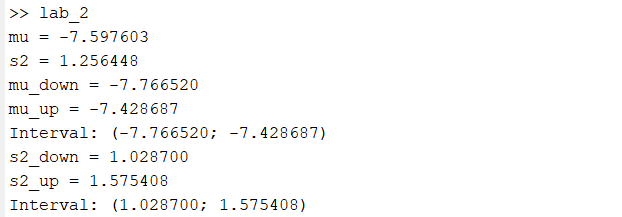
\includegraphics[width=\textwidth]{img/res.png}
	\caption{Результаты расчетов для выборки из индивидуального варианта}
\end{figure}

\begin{figure}[H]
	\centering
	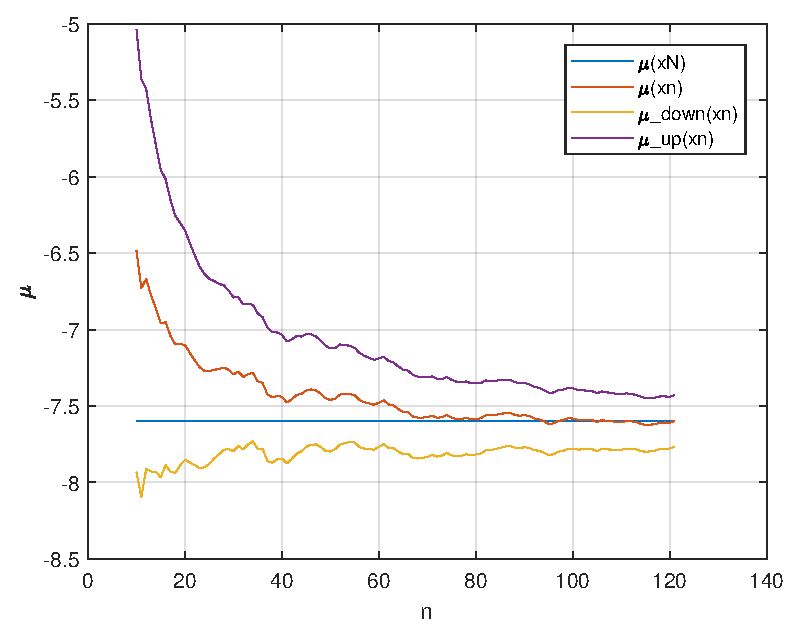
\includegraphics[width=\textwidth]{img/graph1.pdf}
	\caption{График для математического ожидания}
\end{figure}

\begin{figure}[H]
	\centering
	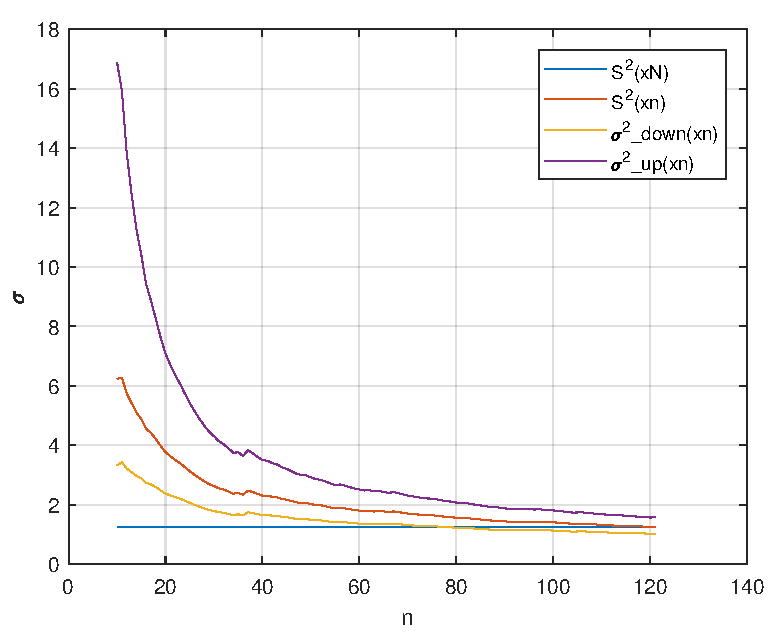
\includegraphics[width=\textwidth]{img/graph2.pdf}
	\caption{График для дисперсии}
\end{figure}

\end{document}